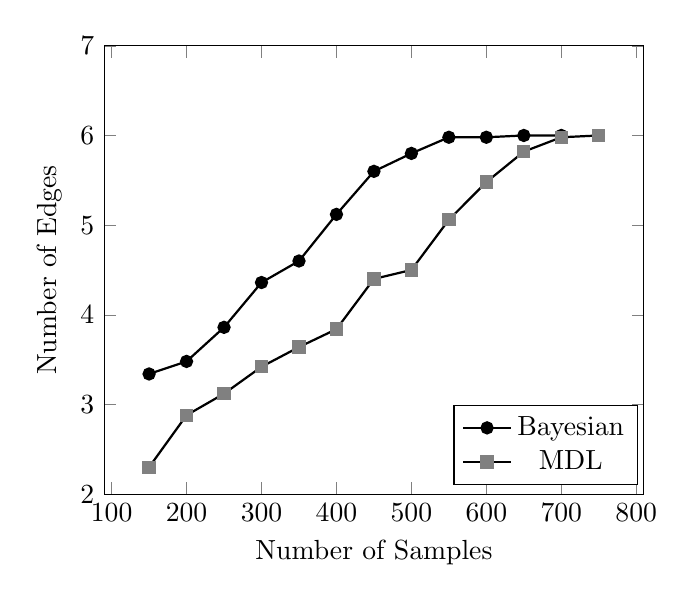
\begin{tikzpicture}
\begin{axis}[
		xlabel = Number of Samples,
		ylabel = Number of Edges,
		legend style={at={(0.99,0.02)},anchor=south east},
		ymin= 2, ymax= 7
]
\addplot+[solid ,black,thick, mark options={black}] coordinates {
(150, 3.34)
(200, 3.48)
(250, 3.86)
(300, 4.36)
(350, 4.6)
(400, 5.12)
(450, 5.6)
(500, 5.8)
(550, 5.98)
(600, 5.98)
(650, 6.0)
(700, 6.0)
};
\addlegendentry{Bayesian};

\addplot+[solid ,black,thick, mark options={black!50}] coordinates {
(150, 2.3)
(200, 2.88)
(250, 3.12)
(300, 3.42)
(350, 3.64)
(400, 3.84)
(450, 4.4)
(500, 4.5)
(550, 5.06)
(600, 5.48)
(650, 5.82)
(700, 5.98)
(750, 6.0)
};
\addlegendentry{MDL};
\end{axis}
\end{tikzpicture}
